\subsubsection{Semi-supervised learning: leveraging real unlabeled resections}
\label{sec:results_semi}

\newcommand{\pseudo}{\st{pseudo}}

In this experiment, we assessed the ability of semi-supervised learning to improve the performance of our baseline model.
We first computed the uncertainty $u(f_{\alpha\beta}, \X\post, n\st{unc})$ for $D\unl$ (\cref{sec:leveraging_semi}), all unlabeled images in EPISURG, using the baseline model and the preprocessing and augmentation transforms (\cref{sec:preprocessing_augmentation}).
We generated pseudolabels and estimated uncertainty from $n\st{unc} = 50$ Monte Carlo \ac{TTA} iterations (\cref{sec:leveraging_semi}).
To obtain the final dataset $D\pseudo = \{ (\X_{\text{postop}_i}, \wt{\Y}_{\text{cavity}_i}) \}_{i = 1}^{n\pseudo}$, we selected pseudolabels with $u(\X_{\text{postop}_i}, \cdot) < t\st{unc} = 0.2$, resulting in $n\pseudo = 256$.

We used $D\st{pre,train}$ (\cref{sec:self}) in addition to $D\pseudo$ to train a new model $\fp{sim,semi}(\cdot)$, using the same hyperparameters as in the self-supervised setting (\cref{sec:self}).
To ensure that all batches contain real resections, we use $b - b\pseudo$ images from $D\st{pre,train}$ and $b\pseudo$ images from $D\pseudo$ to compose each mini-batch of size $b$.
We chose $b\pseudo = 2$ for our experiments, i.e., 20\,\% of the images in each mini-batch contain real resection cavities.

Semi-supervised learning improved the performance of the baseline model from 80.5 (18.7) to 81.5 (17.8) ($p = 0.474$).


\begin{figure}
  \centering

  \begin{subfigure}{0.18\linewidth}
    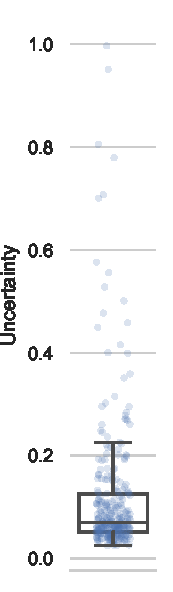
\includegraphics[width=\linewidth]{qcd}
    \caption{\label{fig:all_uncertainties}}
  \end{subfigure}
  \begin{subfigure}{0.194\linewidth}
    \begin{tabular}{c}
      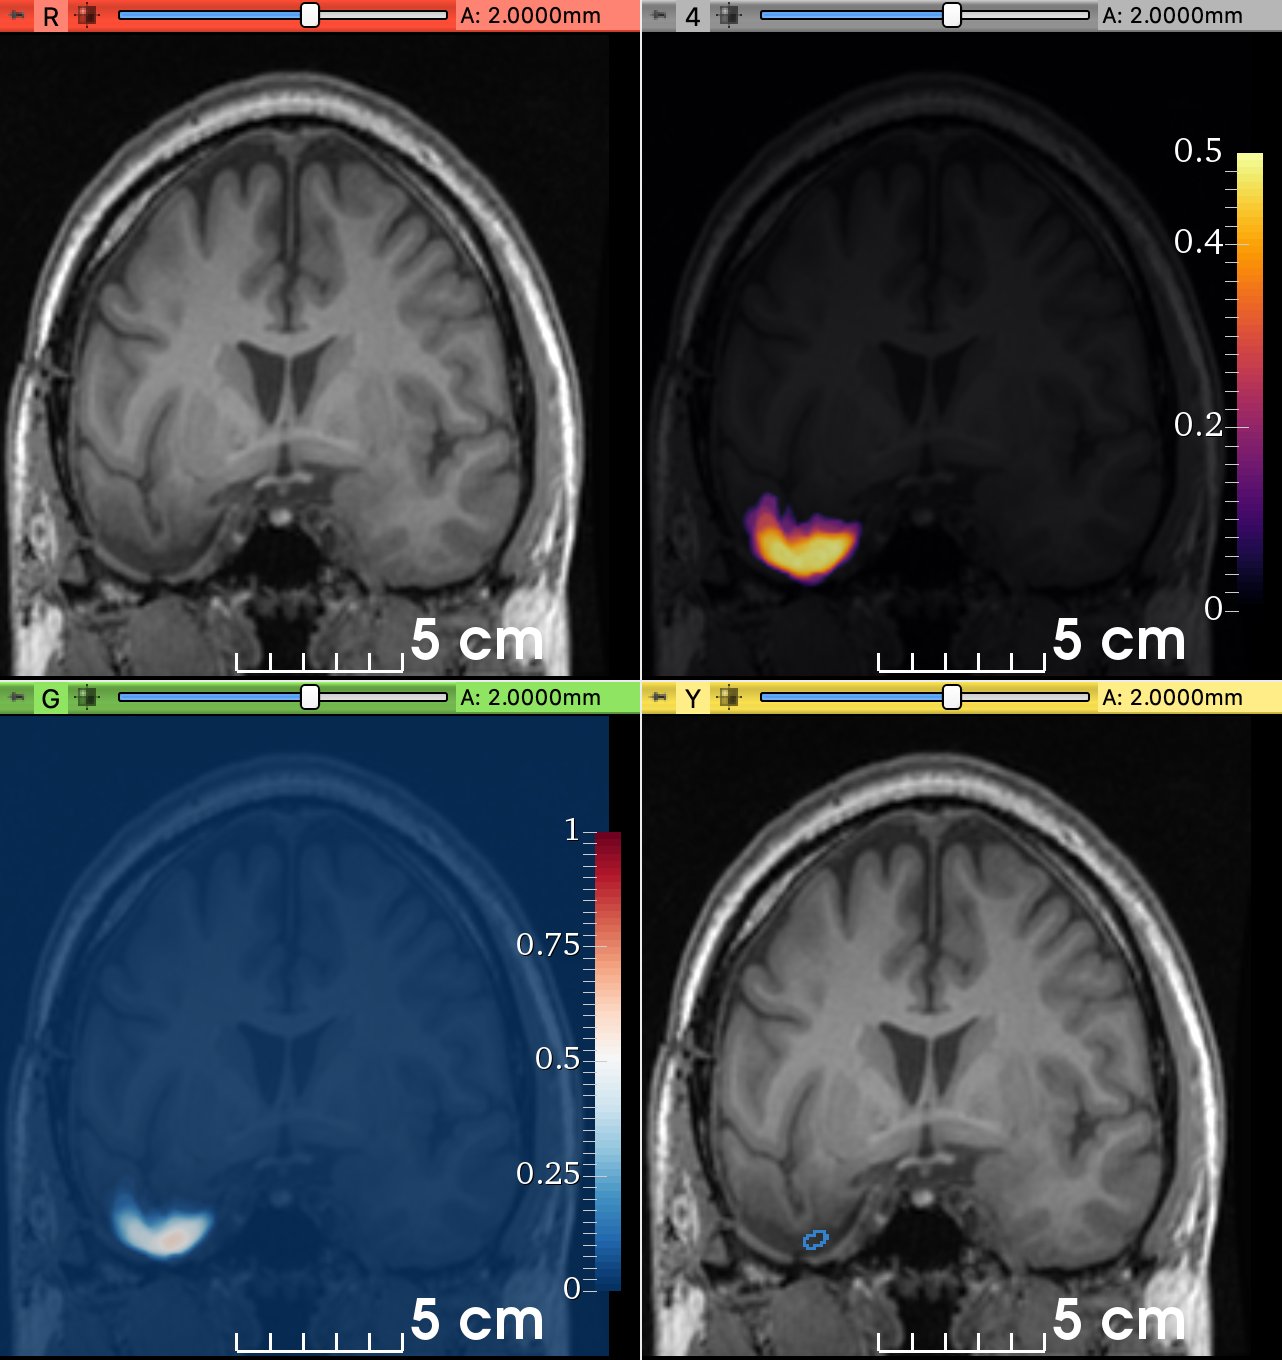
\includegraphics[trim=0 680 642 32, clip, width=\linewidth]{0796_uncertainty} \\
      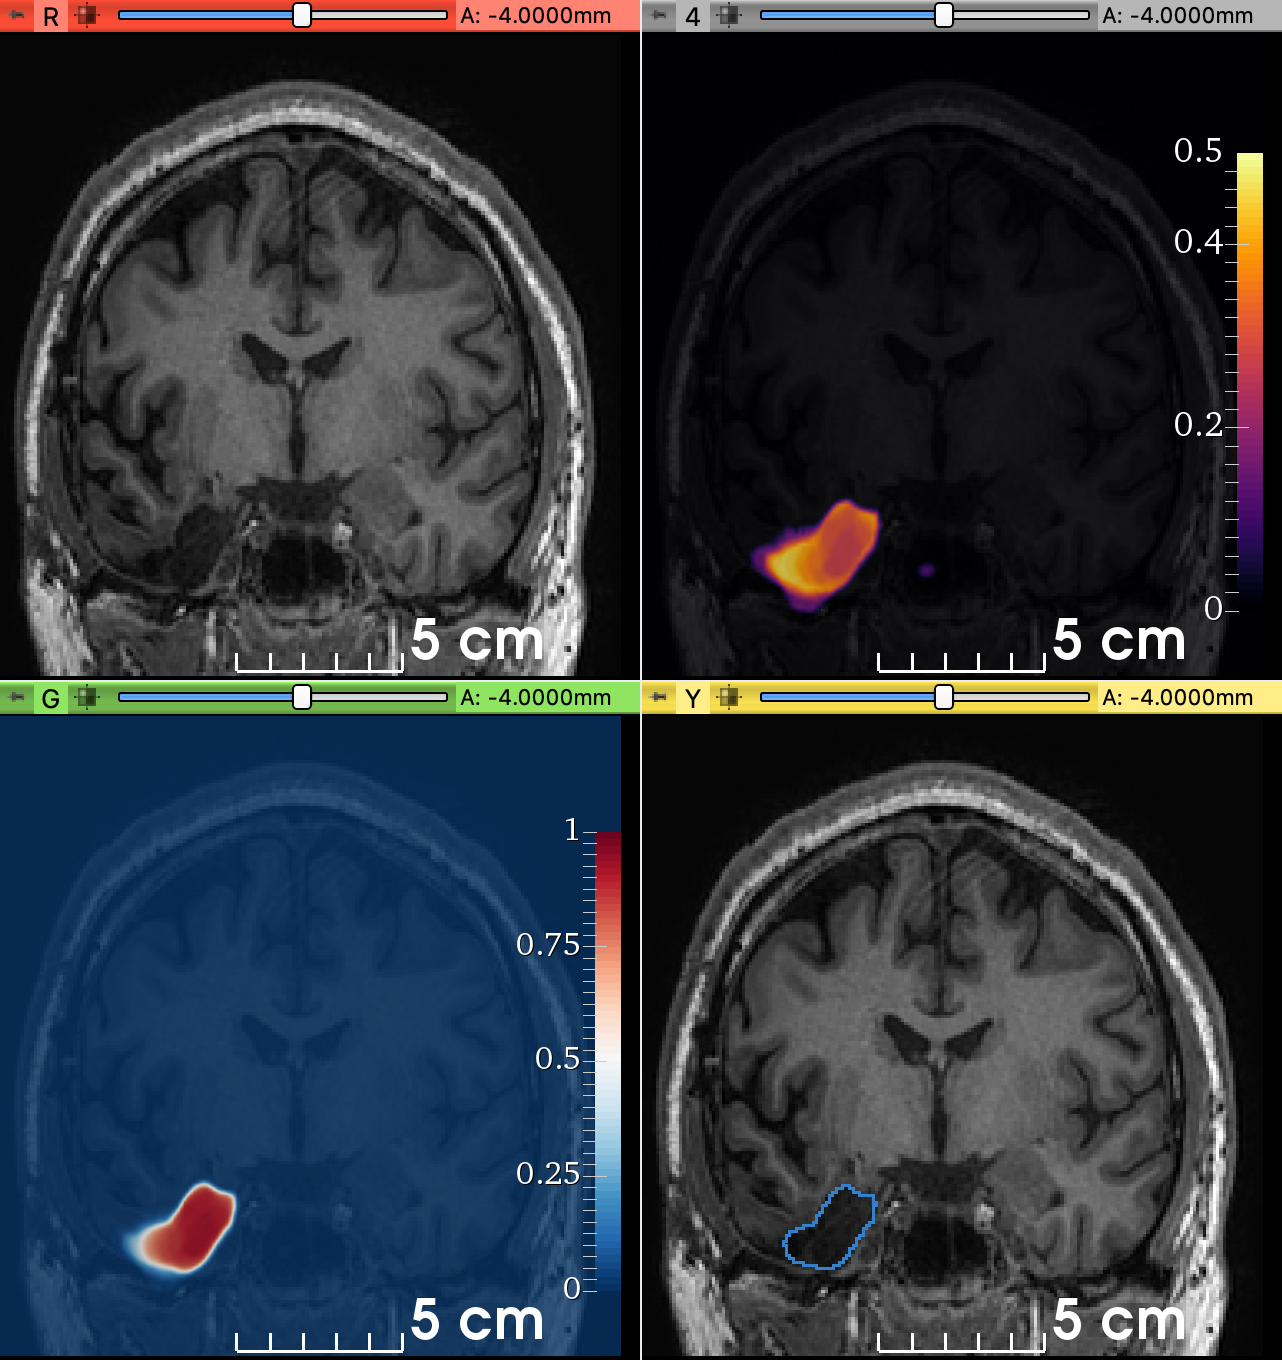
\includegraphics[trim=0 680 642 32, clip, width=\linewidth]{0914_uncertainty} \\
      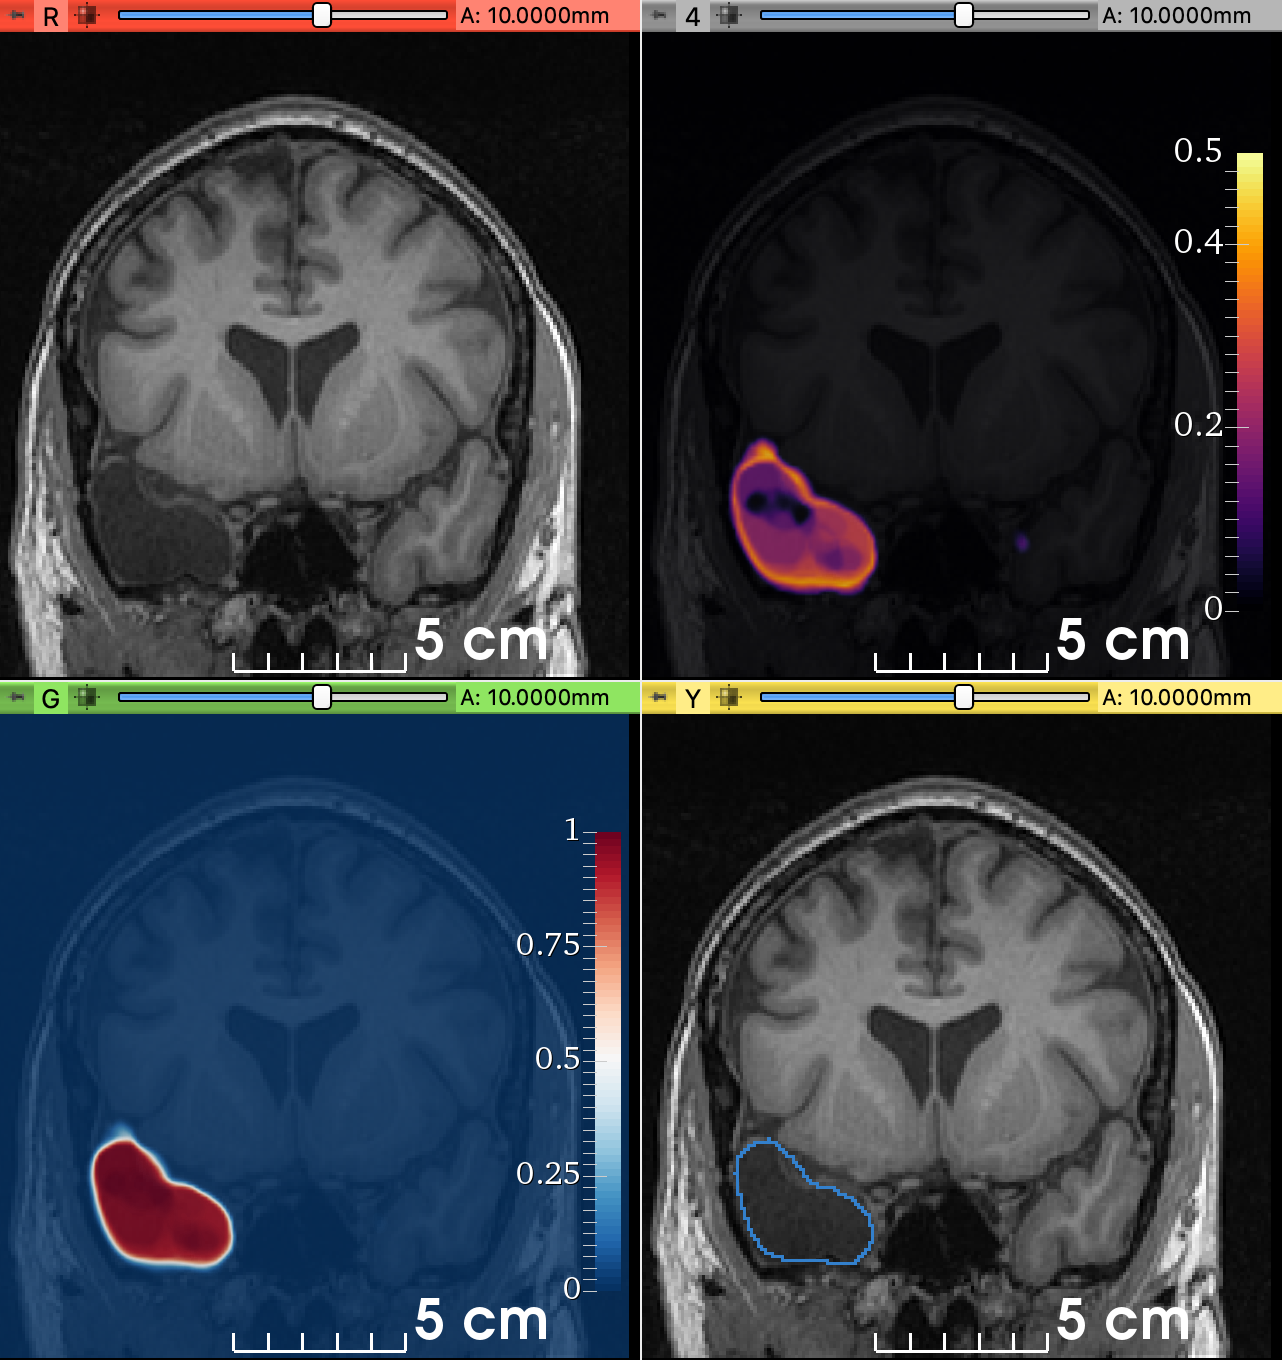
\includegraphics[trim=0 680 642 32, clip, width=\linewidth]{0499_uncertainty} \\
    \end{tabular}
    \caption{\label{fig:uncertainty_mri}}
  \end{subfigure}
  \begin{subfigure}{0.194\linewidth}
    \begin{tabular}{c}
      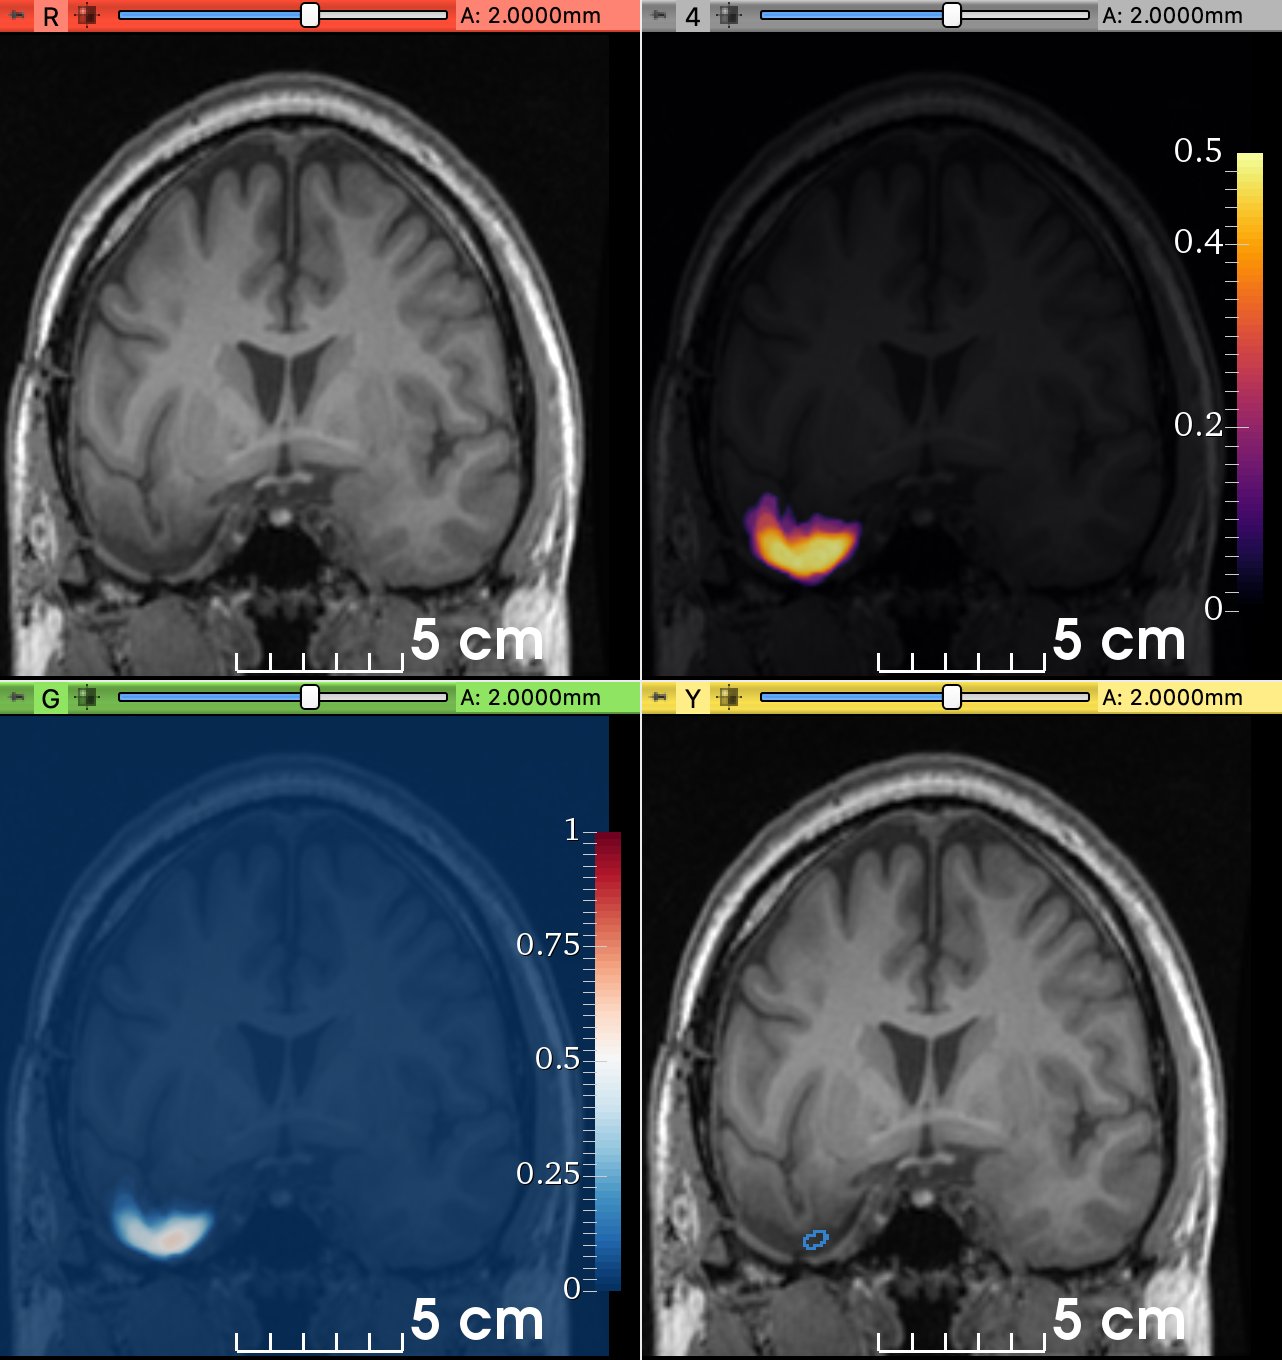
\includegraphics[trim=642 680 0 32, clip, width=\linewidth]{0796_uncertainty} \\
      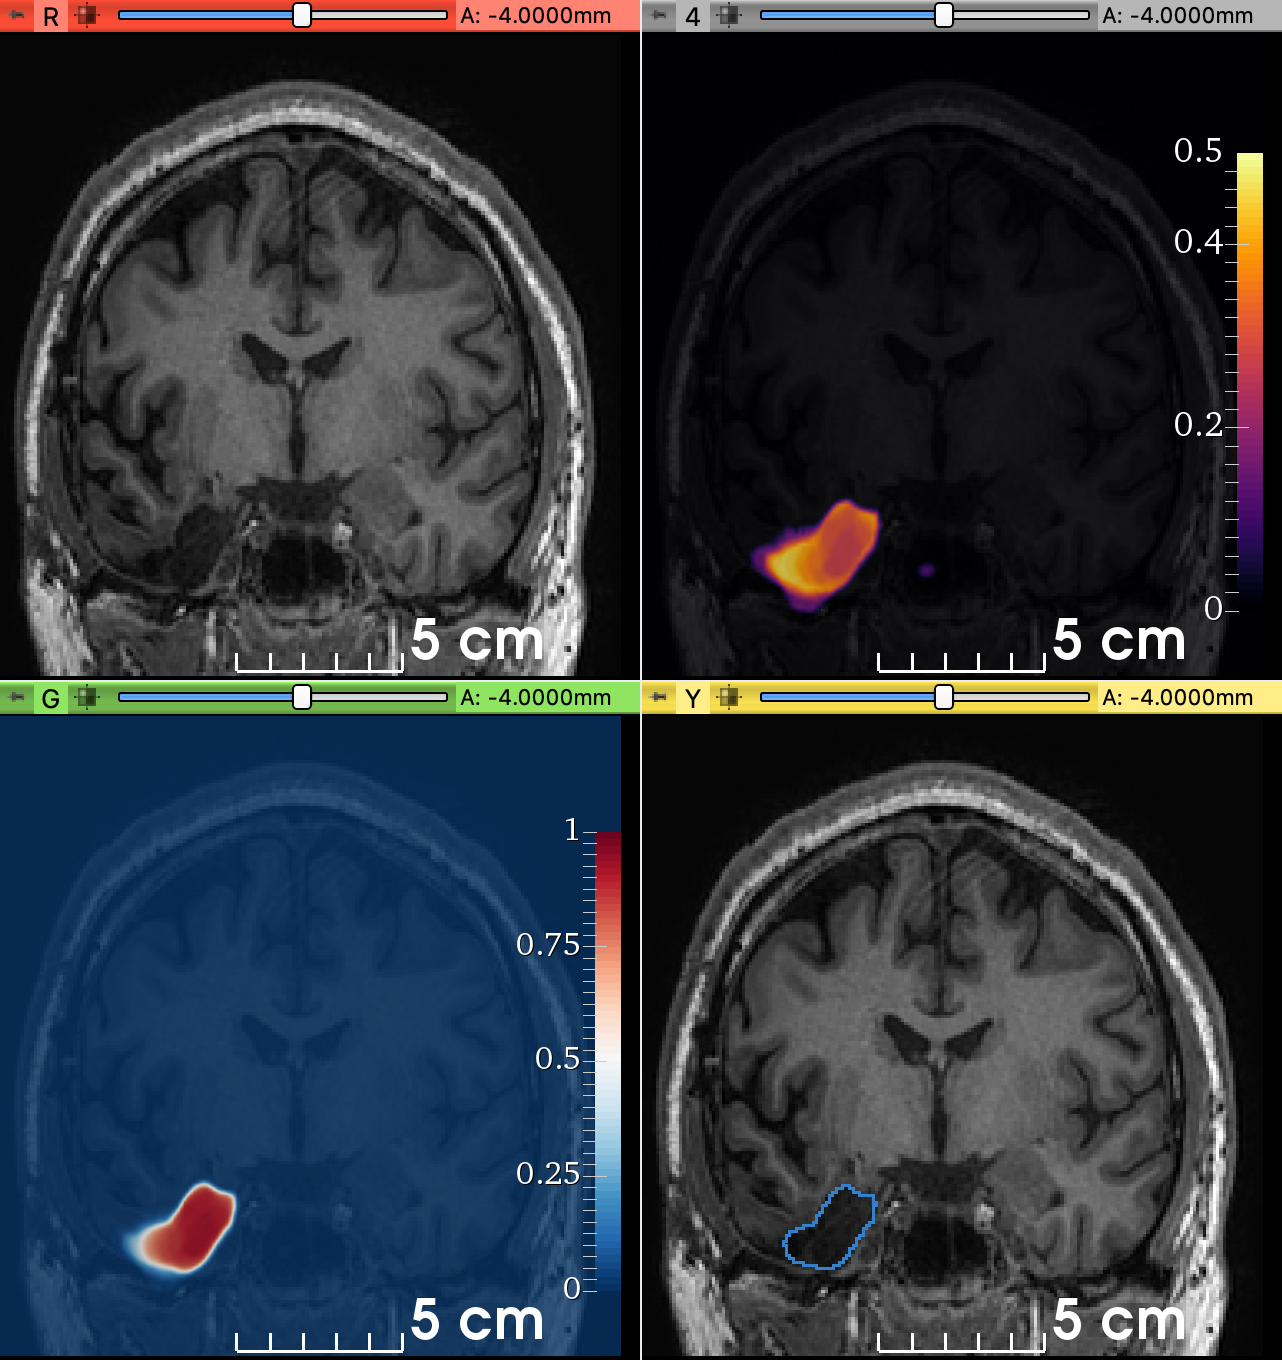
\includegraphics[trim=642 680 0 32, clip, width=\linewidth]{0914_uncertainty} \\
      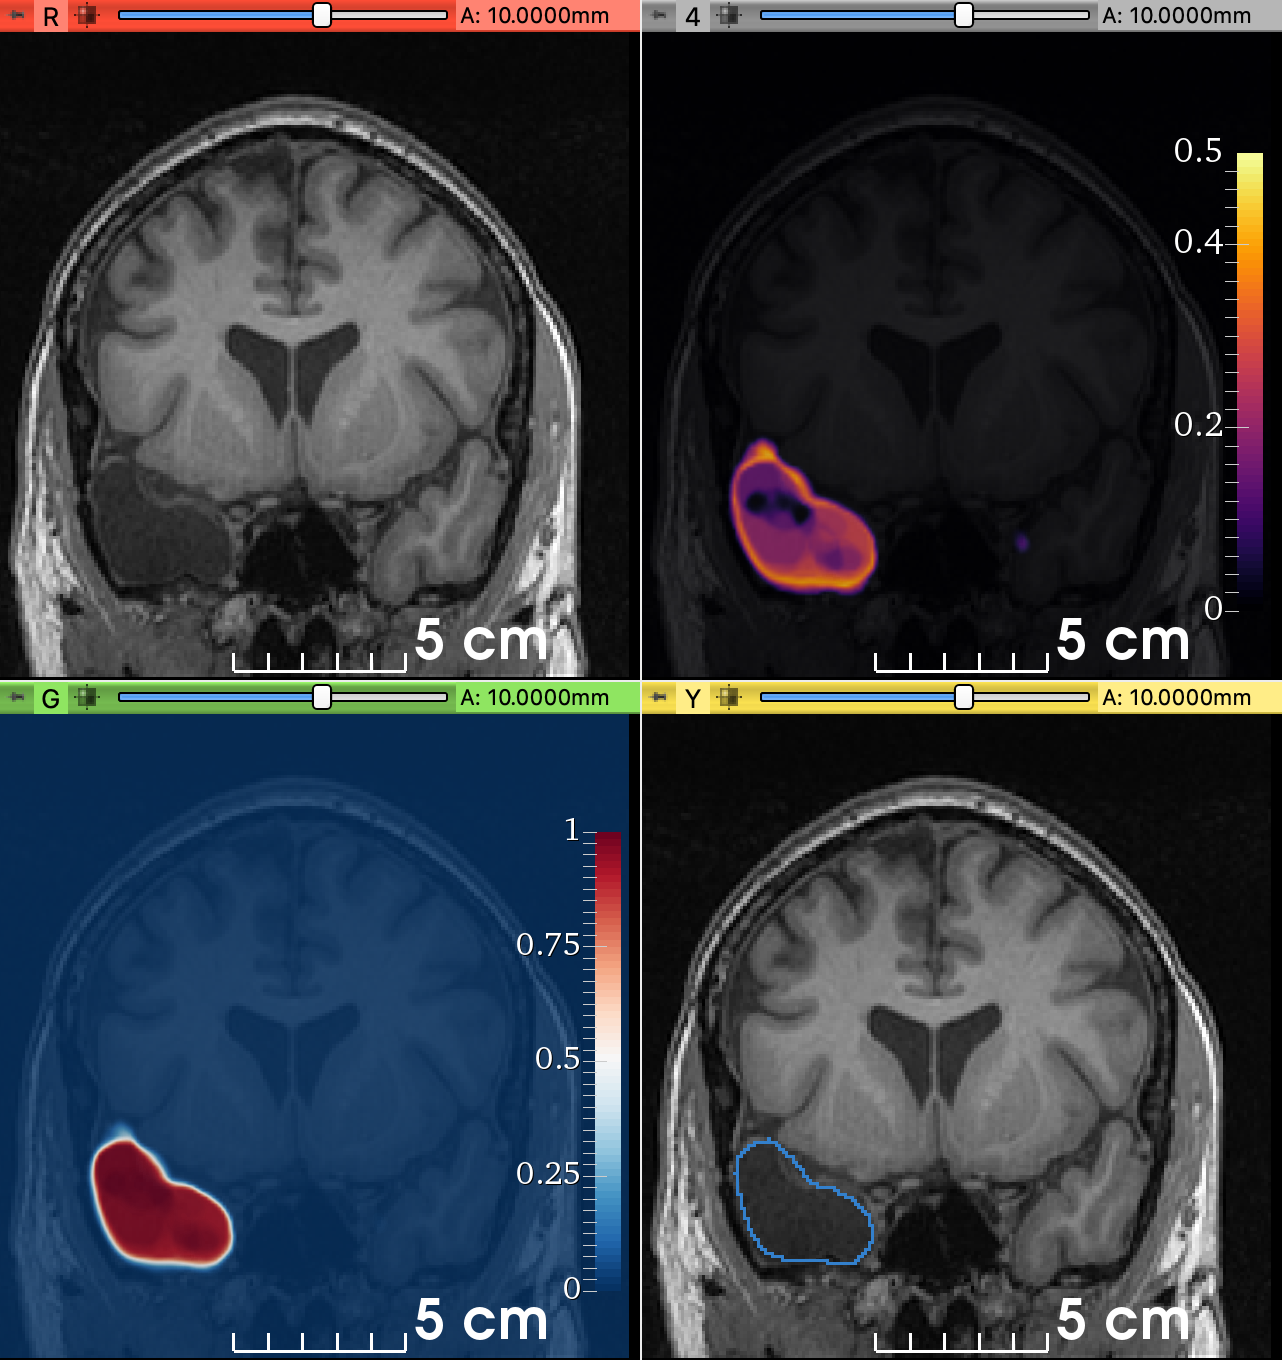
\includegraphics[trim=642 680 0 32, clip, width=\linewidth]{0499_uncertainty} \\
    \end{tabular}
    \caption{\label{fig:uncertainty_std}}
  \end{subfigure}
  \begin{subfigure}{0.194\linewidth}
    \begin{tabular}{c}
      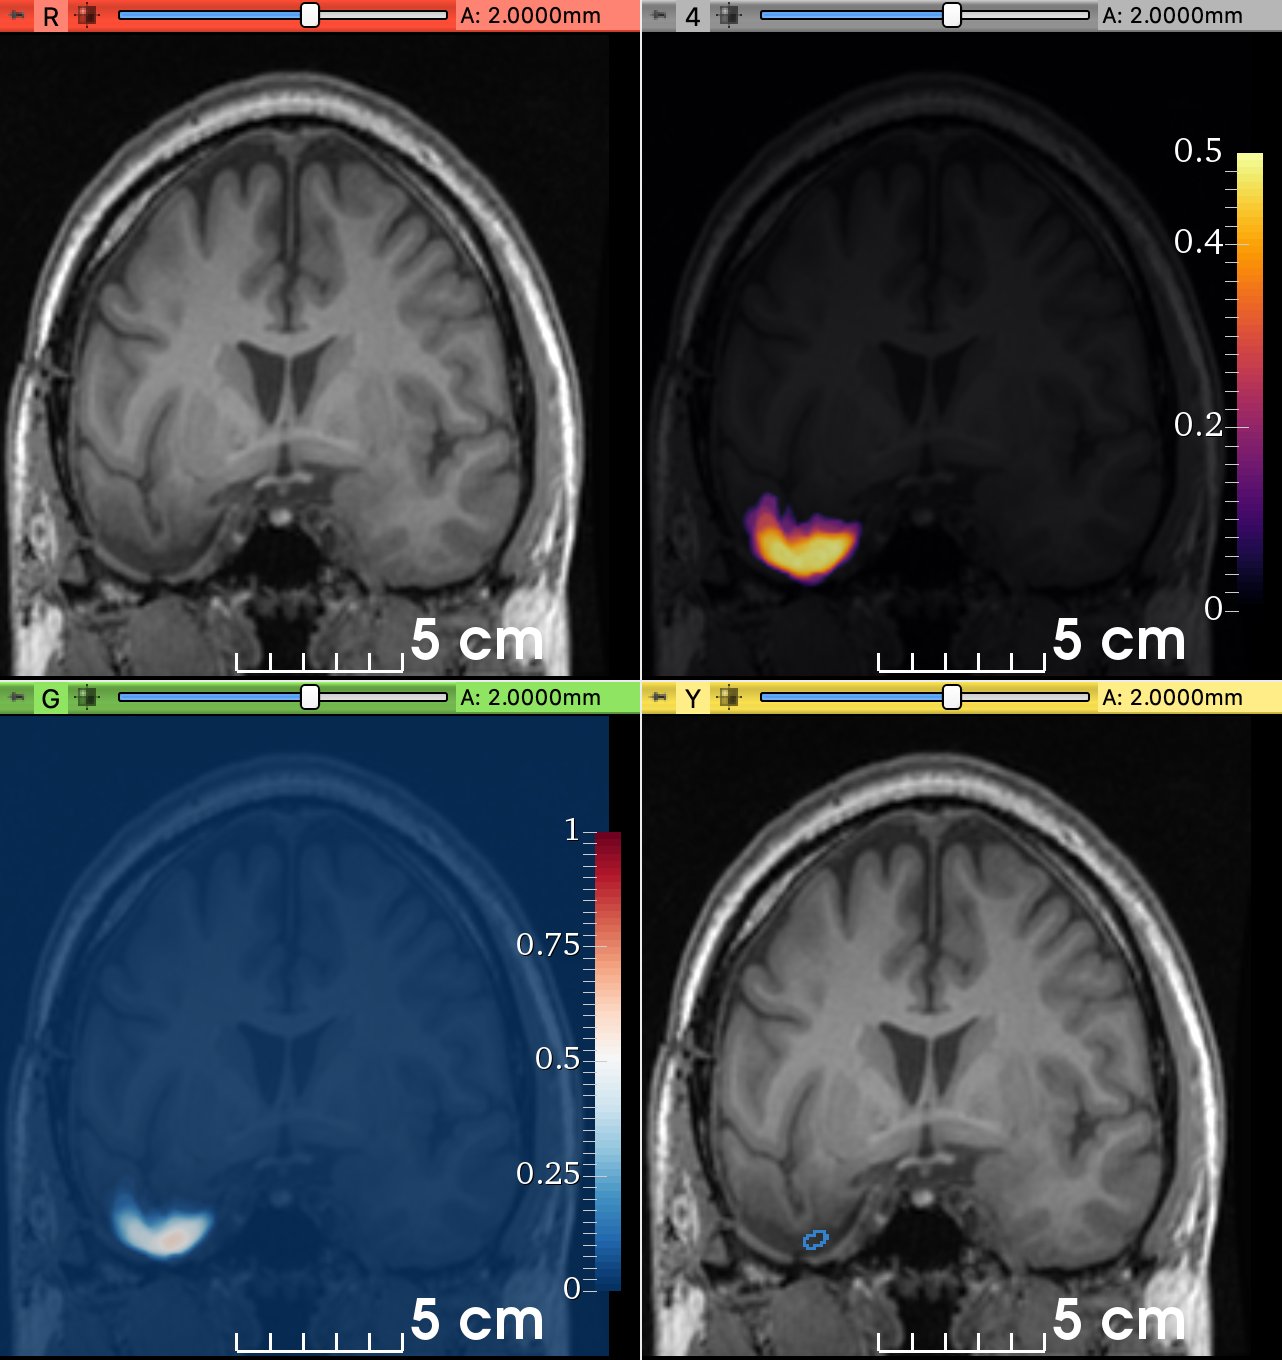
\includegraphics[trim=0 0 642 714, clip, width=\linewidth]{0796_uncertainty} \\
      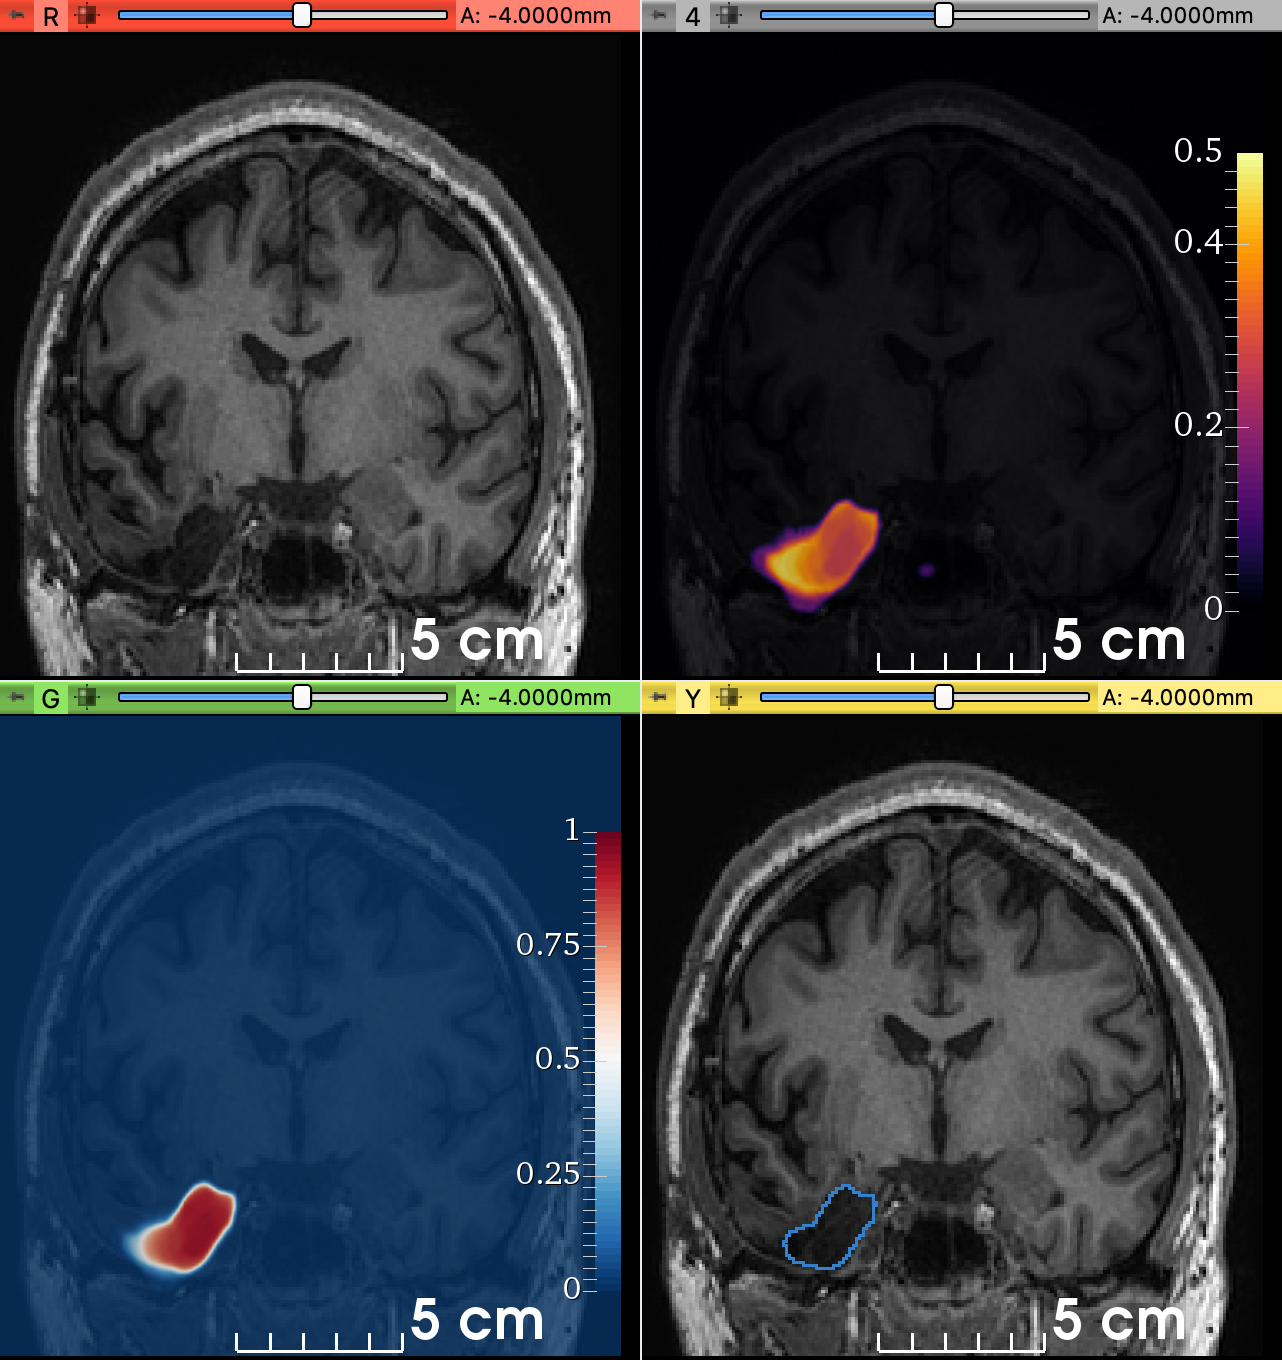
\includegraphics[trim=0 0 642 714, clip, width=\linewidth]{0914_uncertainty} \\
      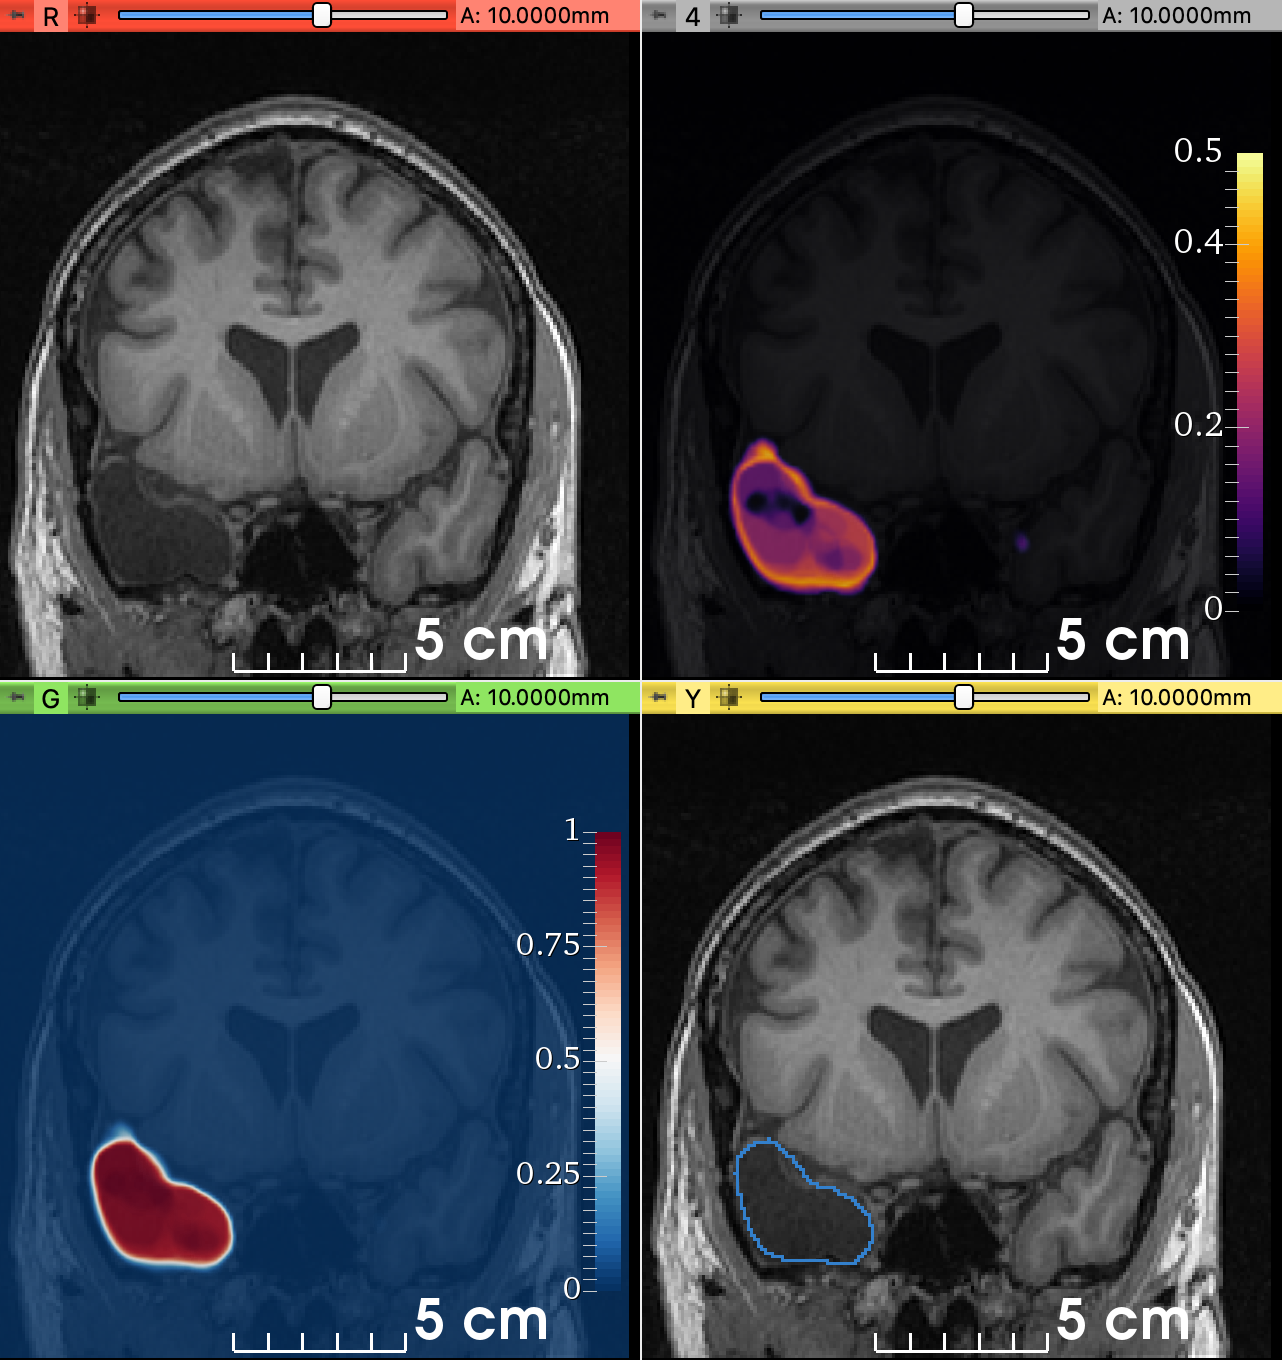
\includegraphics[trim=0 0 642 714, clip, width=\linewidth]{0499_uncertainty} \\
    \end{tabular}
    \caption{\label{fig:uncertainty_mean}}
  \end{subfigure}
  \begin{subfigure}{0.194\linewidth}
    \begin{tabular}{c}
      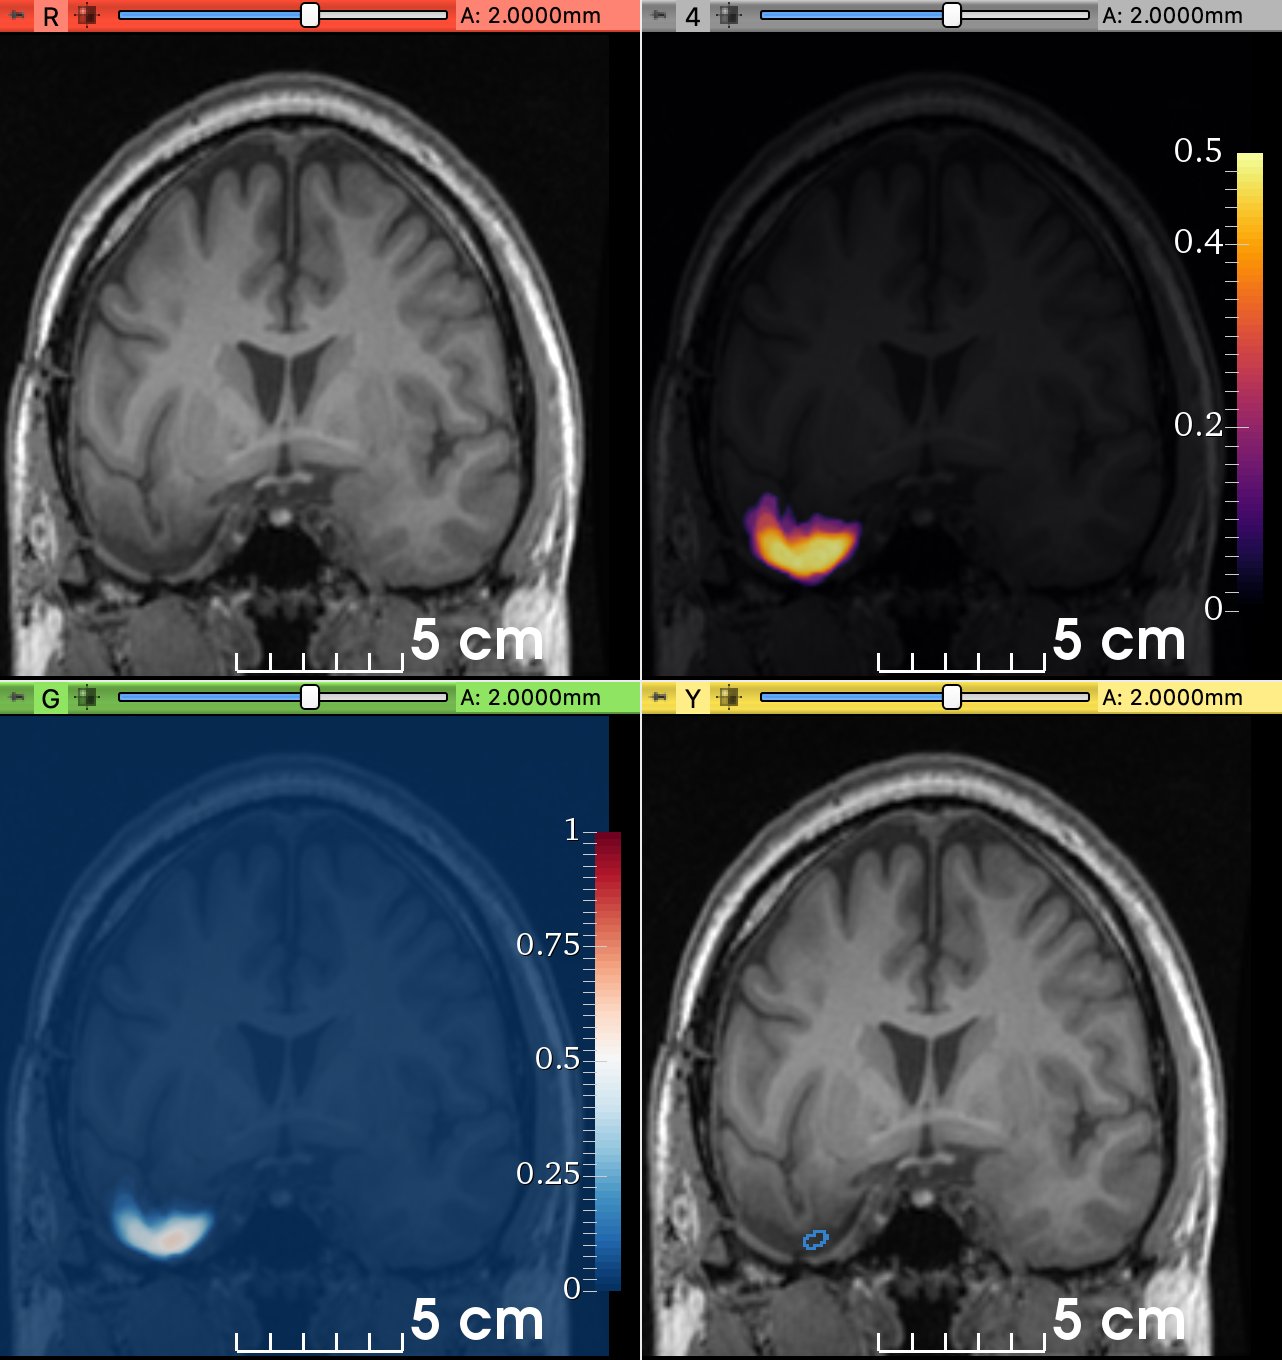
\includegraphics[trim=642 0 0 714, clip, width=\linewidth]{0796_uncertainty} \\
      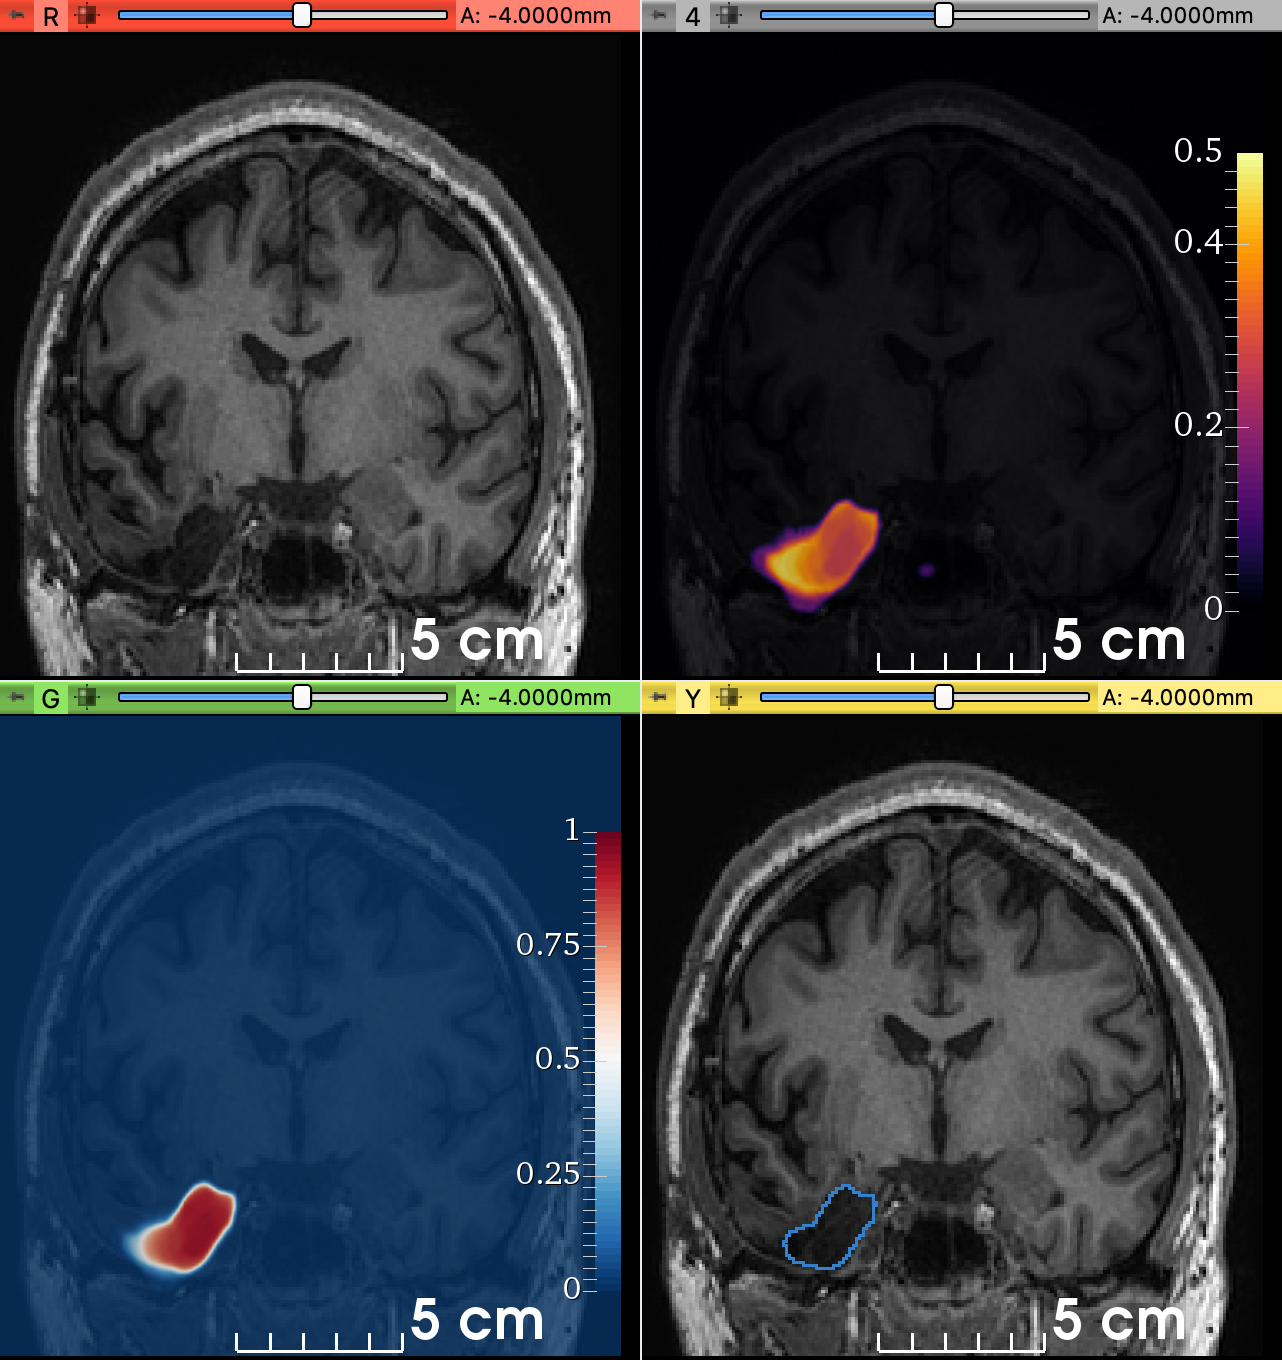
\includegraphics[trim=642 0 0 714, clip, width=\linewidth]{0914_uncertainty} \\
      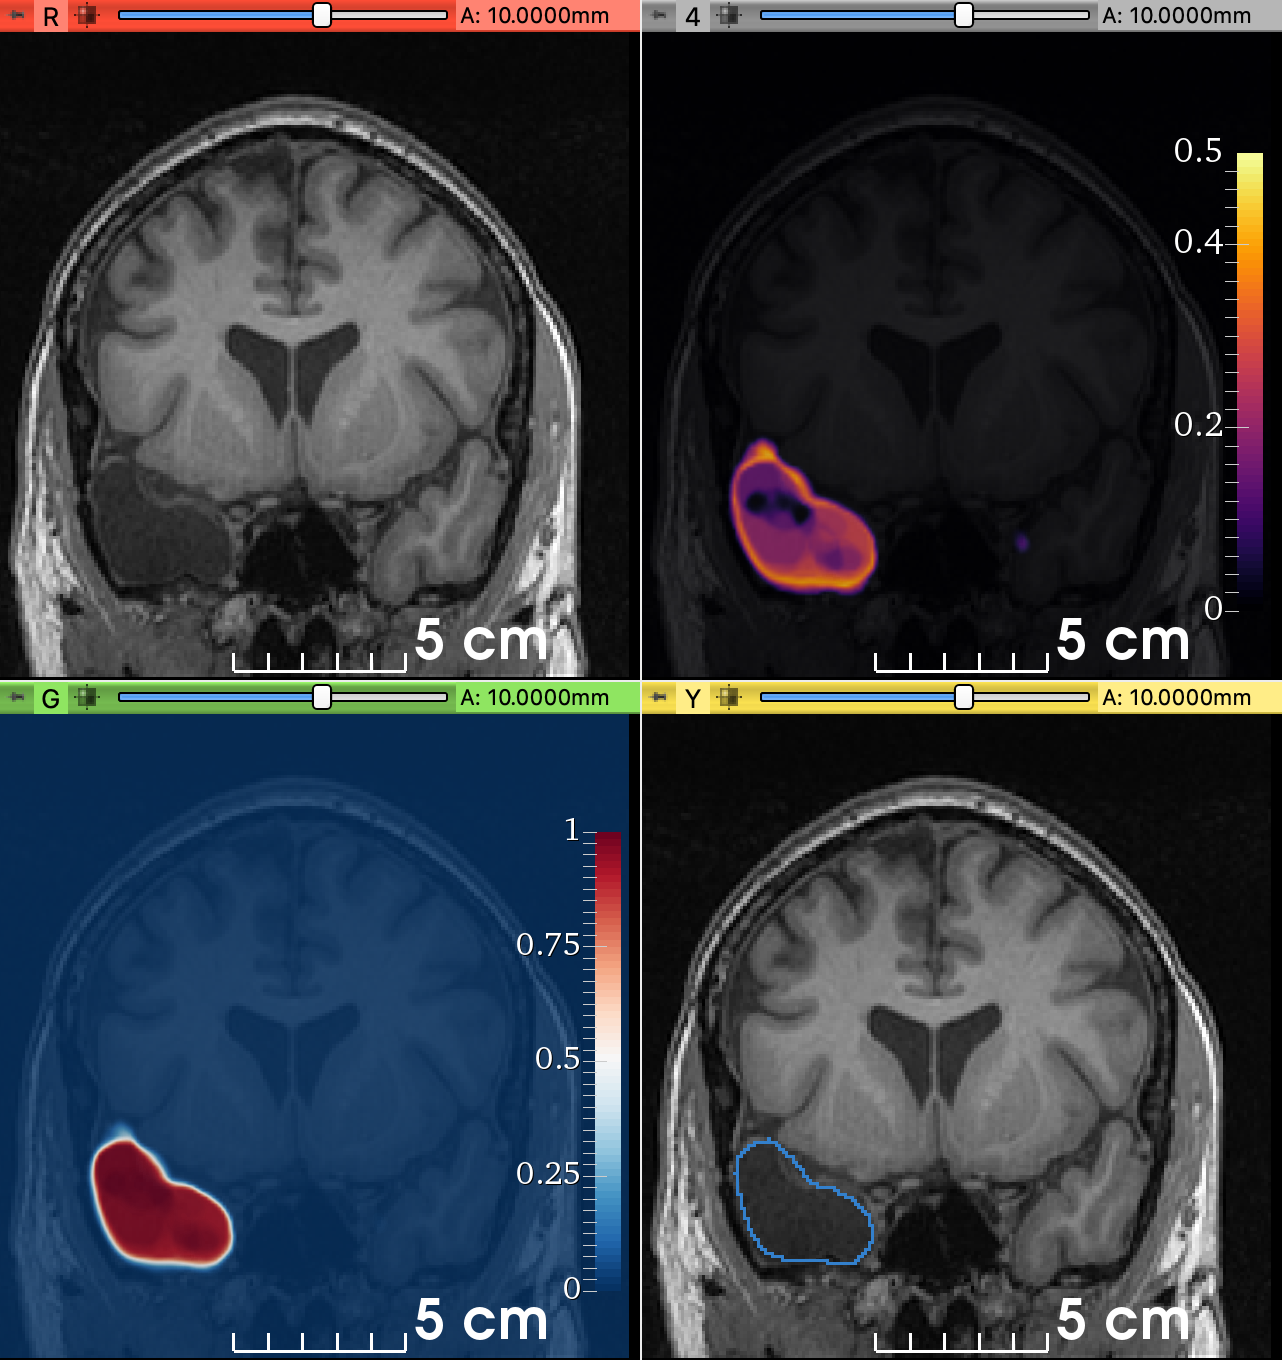
\includegraphics[trim=642 0 0 714, clip, width=\linewidth]{0499_uncertainty} \\
    \end{tabular}
    \caption{\label{fig:uncertainty_pseudo}}
  \end{subfigure}

  \caption[Generating reliable pseudolabels for semi-supervised learning]{
    Generating reliable pseudolabels for semi-supervised learning.
    Image-level uncertainty for the 297 unlabeled postoperative images in EPISURG (\subref{fig:all_uncertainties}).
    Unlabeled postoperative \acf{T1w} \ac{MRI} (\subref{fig:uncertainty_mri}).
    Voxel-wise uncertainty (\subref{fig:uncertainty_std}) estimated as the standard deviation of the probabilities across all Monte Carlo iterations.
    The mean prediction (\subref{fig:uncertainty_mean}) is thresholded at 0.5 to generate the pseudolabel (\subref{fig:uncertainty_pseudo}).
    Image-level uncertainties for the three cases are 0.805 (top), 0.195 (middle) and 0.025 (bottom).
  }
  \label{fig:uncertainties}
\end{figure}
